\documentclass{beamer}
\mode<presentation>{}
\usepackage[utf8]{inputenc}
\usepackage[english]{babel}
\usepackage{hyperref}
\usepackage{verbatim}
\usepackage{listings}
\usepackage{mathabx}
\usepackage{latexsym}
\usepackage{amsmath}
\usepackage{fancyvrb}
\usepackage{graphicx}

\setbeamercovered{invisible}
\usetheme{Frankfurt}
\usefonttheme{serif}

\newcommand{\q}[1]{\texttt{#1}}
\title{Curry\\ Integrating Logic and Functional Paradigms}
\author{Santiago Palacio-Gómez}



\institute{Universidad EAFIT\\Seminario de L\'ogica y Computaci\'on}
\date{\today}


\AtBeginSection[]
{
  \begin{frame}[allowframebreaks]{Table of Contents}
    \tableofcontents[currentsection]
  \end{frame}
}


\begin{document}

\SaveVerb{succ}=Success=
\begin{frame}
  \titlepage
\end{frame}



\begin{frame}
  I do not take credit for the content here. All the research on this matter was made by Michael Hanus and partners. I only intend to make a summary, of what I think are the most important aspects of the language; all with educational purposes.
\end{frame}
\begin{frame}[allowframebreaks]
  \tableofcontents
\end{frame}


\begin{section}{Introduction}
  
  \begin{frame}
    Curry related first paper was published in 1995, by Michael Hanus, Herber Kuchen and Juan Jos\'e Moreno-Navarro, for the International Logic Programming Symposium in 1995, Workshop on Visions for the Future of Logic Programming.
  \end{frame}
\end{section}



\begin{section}{Main Elements}
\begin{frame}
\frametitle{\secname}
  From functional languages, curry takes elements such as:
\begin{itemize}
  \item Expressions.
  \item Functions, high order functions.
  \item Types.
  \item Scope (where clauses, let clauses).
\end{itemize}
\end{frame}
\end{section}

\begin{section}{Narrowing}
  \begin{subsection}{Basic Definitions}
\begin{frame}
\frametitle{\subsecname}
  From the definitions in pure functional programming, we borrow
  \begin{itemize}
    \item Function definition.
    \item Constructors.
    \item Patterns
    \item TRS (\textit{term rewriting system}).
  \end{itemize}


\end{frame}

\begin{frame}
[fragile]
\frametitle{TRS}
 It's worth remembering the definition of a TRS as a set of rewriting rules of the form $l \rightarrow r$ with linear pattern $l$ as $lhs$ and a term r as $rhs$.

  It must also be noticed that the traditional definition of the TRS was changed, by not requiring that $var(l) \subseteq var(r)$.

\begin{example}
\begin{verbatim}
add Z y = y
add (S x) y = S (add x y)
\end{verbatim}
\end{example}

\end{frame}

\begin{frame}
[fragile]

\frametitle{Basic Definitions II}
  We will also take the definitions of position $p$ in a term $t$ ($t|_p$), term replacement $t[s]_p$ and substitutions.

\bigskip
  A term $t$ is called \textit{irreducible} or in \textit{normal form} if there is no term $s$ such that $t \rightarrow s$.
\end{frame}
\end{subsection}

\begin{subsection}{Rewrite Strategy}

  \begin{frame}
\frametitle{\subsecname}
  The goal of a sequence of rewrite steps is to compute a normal form. A \textit{rewrite strategy} determines for each step a rule and a position to apply the next step. A \textit{normalizing strategy} is one that terminates a rewrite sequence in a normal form, when it exists.
\end{frame}

\begin{frame}[fragile]

\frametitle{Constructor Rooted Normalized Form}
Sometimes, the result itself could not be important. For example take the function

\begin{example}
\begin{verbatim}
idNil [] = []
\end{verbatim}
\end{example}
If we try to find the normal form of \verb|idNil[1+2]| we would get \verb|idNil[3]| as normal form.

So, the interesting results of functional computations are \textit{constructor terms} or \textit{values}.
\end{frame}

\begin{frame}
[fragile]

\frametitle{Narrowing}

Functional logic languages are more flexible than pure functional languages since they instantiate variables in a term (free variables), in order to apply the rewrite step. The combination of variable instantiation and rewriting is called \textbf{narrowing}.
\begin{example}
\begin{verbatim}
last :: [a] -> a
last x
     | _++[e] =:= x = e
\end{verbatim}
\end{example}
\end{frame}

\end{subsection}

\begin{subsection}{Formal Definition}
\begin{frame}
\frametitle{\subsecname}
  Formally, $t \leadsto _{p,R,\sigma} t'$ is a \textit{narrowing step} if $t|_p$ is not a variable, and $\sigma(t) \rightarrow_{p,R} t'$.


\bigskip
 Since in functional logic languages we are interested in computing values, as well as answers, we say that $t \leadsto ^ * _ \sigma c$ computes the value $c$ with answer $\sigma$, if $c$ is a value.
  \end{frame}
\end{subsection}

  
\begin{frame}
[fragile]

\frametitle{Example}
  Consider the following program, containing the definition of naturals, the add operation and a ``less than or equal'' test.

\begin{example}

\begin{verbatim}
data Nat = Z | S Nat

add Z y = y
add (S x) y = S (add x y)

leq Z _ = True
leq (S _) Z = False
leq (S x) (S y) = leq x y
\end{verbatim}

\end{example}
\end{frame}

\begin{frame}[fragile]
\frametitle{Efficiency}
  Now, consider the initial term \verb|leq v (add w Z)| where v and w are free variables. By applying $leq_1$, v is instantiated to \verb|Z| and the result \verb|True| is computed:

\begin{center}

\verb|leq v (add w Z)| $\leadsto_{\{v\mapsto Z\}}$ \verb|True|
  
\end{center}

However, we could also do the following:

\begin{center}

\verb|leq v (add w Z)| $\leadsto_{\{w\mapsto Z\}}$ \verb|leq v Z| $\leadsto_{\{v\mapsto Z\}}$ \verb|True|
  
\end{center}

But this would not be optimal since it computes the same value as the first derivation with a less general answer.

\end{frame}

\end{section}

\begin{section}{Needed Narrowing}
  \begin{subsection}{Definition}
    \begin{frame}
      \frametitle{\subsecname}
      
      \begin{itemize}
        \item Designed to perform only necessary narrowing steps.
        \item \textit{Lazy} or \textit{demand-driven}.
      \end{itemize}

      \bigskip
      When performing a narrowing step, if an argument expression must be constructor rooted:
      \begin{itemize}
        \item If the corresponding position is a variable, it's non-deterministically instantiated.
        \item If the corresponding position is an expression, it's evaluated to be constructor-rooted.
      \end{itemize}
      
    \end{frame}
  \end{subsection}
\begin{subsection}{Example}

\begin{frame}[fragile]
\frametitle{\subsecname}
Consider again the program of Natural numbers and the expression \verb|leq v (add w Z)|. 

\bigskip
To get every possible result:
\begin{itemize}
  \item How is \verb|v| instantiated?
  \item How is \verb|w| instantiated?
  
\end{itemize}

\end{frame}
\end{subsection}
\begin{subsection}{Inductively Sequential TRS}
  \begin{frame}[allowpagebreaks]
\frametitle{\subsecname}
To simplify the computational process of needed narrowing, Inductively Sequential TRS are defined. We will characterize a \textit{definitional tree} $T$ (using the \textit{subsumption ordering}: $t \leq \sigma (t)$) of an operation $f$ with the following properties. Each property will be exemplified from using the natural numbers example.
\end{frame}
\begin{frame}
[fragile]
\frametitle{Leaves property} The maximal elements of $T$, called the \textit{leaves}, are the lhs of the rules defining $f$.

\begin{example}
  The leaves of \verb|add| are \verb|add Z y| and \verb|add (S x) y|.
\end{example}
\end{frame}
\begin{frame}
[fragile]
\frametitle{Root property}
Has a minimum element, called the \textit{root}, of the form $f(x_1,x_2,\ldots,x_n)$ where $x_1,\ldots\,x_n$ are pairwise distinct variables.

\begin{example}
The root of \verb|add| is \verb|add x y|.

\end{example}
\end{frame}
\begin{frame}
[fragile]
  \frametitle{Parent property} For every pattern $\pi$ different from the root, there exists a unique $\pi'$, the parent, such that $\pi' < \pi$ and there isn't any $\pi''$ such that $\pi' < \pi'' < \pi$.

\begin{example}
  \verb|leq x y| could* be parent of \verb|leq (S x') y| and \verb|leq x (S x')|; however, it is not the parent of \verb|leq (S x') (S y')|.
\end{example}
\end{frame}
\begin{frame}
[fragile]
\frametitle{Induction property} Every child of $\pi$ differs from each other only at a common position, called the \textit{inductive position}, which is the position of a variable in $\pi$.

\begin{example}
\verb|leq (S x) y| and \verb|leq Z y| could be siblings; however \verb|leq (S x) y| and \verb|leq x (S y)|, differ in two positions, thus could not be siblings.
\end{example}

\end{frame}
\begin{frame}
\frametitle{Inductively sequential TRS II}
\begin{itemize}
\item An operation is called inductively sequential if it has a definitional tree and its rules do not contain extra variables.
\item A TRS is inductively sequential if every define operation is inductively sequential. 
\end{itemize}
\end{frame}

\begin{frame}
[fragile]

\frametitle{Applicability}
Needed narrowing is applicable to many operations in logic functional languages (and every operation in pure functional languages), however extensions may be useful for particular operations.

\begin{example}
\begin{verbatim}
or _ True = True
or True _ = True
or False False = False
\end{verbatim}
\end{example}
\end{frame}

\begin{frame}

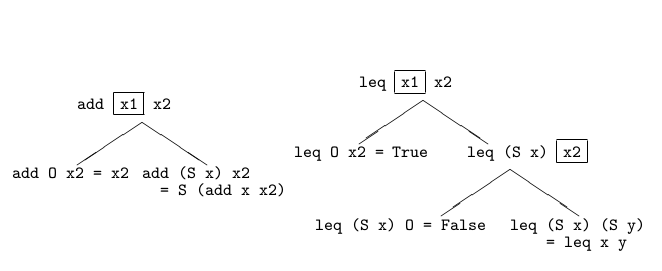
\includegraphics[scale=0.5]{pictures/def_trees.png}
  
\end{frame}

\begin{frame}
\frametitle{Use of Definitional Trees in Narrowing}

  Definitional Trees can be computed at compile time and they contain all information for the decisions to the steps in the rewriting process.

  We could define a needed narrowing step as an application to an operation-rooted term $t$ by considering it's definitional tree. First, we find the \textit{maximal} node $pi$ that unifies with $t$, and applies the following algorithm.

\end{frame}

\begin{frame}
\frametitle{Needed Narrowing Algorithm}
  \begin{itemize}
%    \setlength{\itemindent}{2cm}
\item If $\pi$ is a leaf, we apply the corresponding rule
\item If $\pi$ is a branch, let p be it's inductive position, we consider the corresponding subterm$t|_p$
  \begin{itemize}
  \item If $t|_p$ is rooted by a constructor $c$, if there is a child  with $c$ at the inductive position, we examine the child, else we fail.

  \item If $t|_p$ is a variable, we non-deterministaclly instantiate this variable by the constructor term at the inductive position of a child, and proceed to examine the child.

  \item If $t|_p$ is operation rooted, we recusively apply the computation of a needed narrowing step to $\sigma(t|_p)$, where $\sigma$ is the substitution, result of previous case distinctions.
  \end{itemize}
\end{itemize}

\end{frame}
\end{subsection}
\begin{subsection}{Strict Equality}
\begin{frame}[fragile]
\frametitle{\subsecname}
    The equality symbol \verb|=:=| is called \textit{strict equality}, i.e. the equation $t_1 =:= t_2$ is satisfied iff $t_1$ and $t_2$ are reducible to the same \textit{ground} constructor or term. (Note that when $t_1$ is not reducible, $t_1 =:= t_1$ does not succeed).

    We can define $=:=$ as follows:

    \[
    \begin{array}{llr}
    
      c =:= c &= \UseVerb{succ} &\forall  c/0\\
      c ~ x_1 \ldots ~ x_n =:= c ~ y_1 \ldots ~ y_n &= x_1 =:= y_1 ~\&~ \ldots x_n =:= y_n &\forall c/n \\
      \UseVerb{succ}~ \&~ \UseVerb{succ} &= \UseVerb{succ}
    \end{array}
    \]
\end{frame}

\begin{frame}[fragile]
\frametitle{Strict Equality Solutions}
A solution for an equation $t_1 =:= t_2$ is a substitution $\sigma$, if $\sigma(t_1) =:= \sigma(t_2) \leadsto^* \UseVerb{succ}$.

We have then, that \textit{needed narrowing} is Correct, Complete and Minimal (if there are two derivations, then their substitutions are independent). And, in successful derivations, needed narrowing computes the \textit{shortest} of all possible narrowing derivations.

\end{frame}
\end{subsection}

\begin{subsection}{Weakly Needed Narrowing}

\begin{frame}[fragile]
\frametitle{\subsecname}
  If we take the previously shown code:
\begin{verbatim}

or _ True = True
or True _ = True
or False False = False

\end{verbatim}

 We must extend the definition of \textit{inductively sequential TRS} to a \textit{weakly orthogonal TRS} by requiring only that, for all variants of rules $\l_1 \rightarrow r_1$, $l_2 \rightarrow r_2$, if $\sigma(l_1) = \sigma(l_2)$ then $\sigma(r_1) = \sigma(r_2)$.

\end{frame}

\begin{frame}
\frametitle{{\subsecname} II}
  Then, we can also extend the definition of \textit{definitional trees} by adding or-branches, which are conceptually the union of two definitional trees.

  In the previous example, we could create a tree for the rules {$or_2,or_3$} and the rule {$or_1$}, then we could join those trees by an or-branch.

  This new way of resolving operations is also confluent, for the condition we required.

  \end{frame}
\end{subsection}
\end{section}
\begin{section}{Non-Determinism}

\begin{subsection}{Handling Non-Determinism}
\begin{frame}[fragile]
\frametitle{\subsecname}
  This same principle may also be extended to handle non-deterministic operations and extra variables, by simply examining every possible or branch, and not requiring that all the rules are confluent to the same normal form. For example, the rule

\begin{verbatim}
x ? _ = x
_ ? y = y
\end{verbatim}

  Gives two results for \verb|0 ? 1|, namely \verb|0| and \verb|1|.
  
\end{frame}

\end{subsection}
\begin{subsection}{Lazy vs Strict Evaluation}
\begin{frame}
[fragile]
\frametitle{\subsecname}
  Consider the following functions
\begin{verbatim}
choose x _ = x
choose _ y = y

coin = choose 0 1

double x = x+x
\end{verbatim}
What would happen if we call \verb|double coin|?.
\end{frame}
\begin{frame}
[fragile]
\frametitle{{\subsecname} Examples}
\begin{example}
\begin{verbatim}
coin = 0 ? 1

double x = x+x


insert e [] = [e]
insert e (x:xs) = (e:x:xs) ? (x : (insert e xs))

perm [] = []
perm (x:xs) = insert x (perm xs)
\end{verbatim}
\end{example}
\end{frame}
\begin{frame}
[fragile]
\frametitle{{\subsecname} Examples II}
\begin{example}
\begin{verbatim}
sorted :: [Integer] -> [Integer]
sorted [] = []
sorted [x] = [x]
sorted (x:y:xs) | ((x < y)::Bool) =:= True 
                  = x : (sorted (y:xs))

mySort x = sorted (perm x)
\end{verbatim}
\end{example}
\end{frame}
\end{subsection}
\end{section}
\begin{section}{Bibliography}
  \begin{frame}
    \frametitle{\secname}
    \begin{itemize}
    \item Curry: A tutorial Introduction. Draft of December 2007. Antoy Sergio, Hanus Michael, Taken from http://www.informatik.uni-kiel.de/~Curry/tutorial/ the 15th of April, 2013.


    \item Functional Logic Programming: From Theory to Curry. Hanus Michael. Institut f\"ur Informatik, CAU Kiel, Germany. As sent May the 13th of 2013.

    \item Curry An integrated functional language. September 11,2012. Hanus Michael, retrieved the 15th of April 2013.

    \item Curry: A truly Integrated Functional Logic Language. December 1995. Hanus Michael, Kuchen Herbert, Moreno-Navarro Juan Jos\'e, retrieved 9th of September 2013.
      
    \end{itemize}

\end{frame}
\end{section}

\end{document}
